% Created 2026-02-27 Fri 09:43
% Intended LaTeX compiler: pdflatex
\documentclass[bigger]{beamer}
\usepackage[utf8]{inputenc}
\usepackage[T1]{fontenc}
\usepackage{graphicx}
\usepackage{grffile}
\usepackage{longtable}
\usepackage{wrapfig}
\usepackage{rotating}
\usepackage[normalem]{ulem}
\usepackage{amsmath}
\usepackage{textcomp}
\usepackage{amssymb}
\usepackage{capt-of}
\usepackage{hyperref}
\usepackage[spanish, mexico]{babel}
\uselanguage{Spanish}
\languagepath{Spanish}
\usepackage{mathtools}
\input{ext-link.tex}
\usetheme[height=20pt]{Rochester}
\usecolortheme{lily}
\author{Eric Magar \newline ITAM}
\date{Tec de Monterrey's PoliSci Conference \newline 27-2-2026}
\title{Is reelection an antidote to the incumbency curse?}
\subtitle{Evidence from Mexican municipal races 1997--2025}
\setbeamertemplate{footline}[frame number]{}
\setbeamertemplate{navigation symbols}{}
\expandafter\def\expandafter\insertshorttitle\expandafter{%
\insertshorttitle\hfill%
\insertframenumber}
%  \insertframenumber\,/\,\inserttotalframenumber}
\hypersetup{
 pdfauthor={Eric Magar \newline ITAM},
 pdftitle={Is reelection an antidote to the incumbency curse?},
 pdfkeywords={},
 pdfsubject={},
 pdfcreator={Emacs 27.1 (Org mode 9.3)}, 
 pdflang={Spanish}}
\begin{document}

\maketitle
\begin{frame}{Outline}
\tableofcontents
\end{frame}

\setbeamercovered{transparent}

\section{Motivation}
\label{sec:orgc792038}
\begin{frame}[label={sec:orgc0f4942}]{Motivation}
\begin{block}{Does winning office improve a party's \newline future electoral fortunes?}
\pause

\bigskip
\begin{itemize}
\item Not in Mexico (Lucardi--Rosas 2016)
\item Coalitions started from scratch at each cycle? \newline (Díaz Cayeros et al. 2016)
\item ``Incumbency curse'' (also in Brazil, India, \ldots{})
\end{itemize}
\end{block}
\end{frame}
\begin{frame}[label={sec:org87e2b85}]{Lucardi--Rosas}
Marginal municipal races 1997--2010, regression discontinuity

\bigskip
\centering
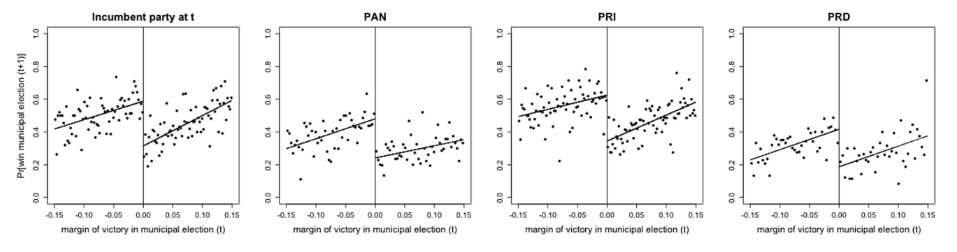
\includegraphics[width=\textwidth]{../../plots/luro-fig1.png} \pause
\begin{block}{Study antedates last decade's \alert{reelection} reform}
\(\rightarrow\) Could this change the curse into an incumbency advantage? \newline  (Erikson 1971, \ldots{})
\end{block}
\end{frame}
\section{The removal of single-term limits}
\label{sec:org2bd40c1}
\begin{frame}[label={sec:orgbbc5f5e}]{Electoral reform}
\begin{block}{Between 2018 and 2030:}
\begin{itemize}
\item Two-term limits for municipal officers \pause
\item Staggered removal of single-term limits: \newline 23 states in 2018, 3 in 2019, 2 in 2021, 2 in 2024 \newline (and 2 non-reformers) \pause
\item Many municipal presidents on the ballot
\end{itemize}
\centering \footnotesize
\bigskip

\begin{tabular}{crrrrrr}
             & Incumbent         & Term       & Open        & Pre-          &       &      \\ [-0.4ex]
  Cycle      &      ran          & limit      & seat        & kick-off      & Total &    N \\ [1ex] \hline \\ [-1.8ex]
  2018--2019 &                32 &          0 &          54 &            14 &   100 & 1,660 \\
  2021--2022 &                36 &         16 &          44 &             5 &   100 & 1,741 \\
  2024--2025 &                45 &         19 &          36 &             0 &   100 & 1,743 \\ [0.5ex] 
  Total      &                38 &         12 &          44 &             6 &   100 & 5,144 \\
  \\ [-2ex] \hline
\end{tabular}
\end{block}
\end{frame}
\begin{frame}[label={sec:orgbe25c0c}]{Minimal effects?}
Motolinia (2026) state legislators
\begin{block}{Relative to rest, members who sought reelection}
\begin{itemize}
\item 2\% likelier to mention pork in speeches
\item spent 15\% more in casework
\item twice likelier to sit in pork committees
\item but no change in party discipline \pause
\end{itemize}
\end{block}
\begin{block}{Might this be different among \alert{executive} officers?}
\end{block}
\end{frame}
\section{Model}
\label{sec:org19c030c}
\begin{frame}[label={sec:org2717196}]{Controlling incumbents on the ballot}
\begin{block}{Switching-regime model:}
\footnotesize
\begin{equation*}
\begin{split}
\text{logit}\bigl(p_{t+1}\bigr) =  & ~~~~~~~~~~~\text{neg}_t~ \times (\alpha_0 + \alpha_1 \text{ocup}_{t+1} + \alpha_2 \text{mg}_t + \alpha_3 \text{ocup}_{t+1} \times \text{mg}_t) \\
                                   & +~ (1 - \text{neg}_t) \times (\beta_0 + \beta_1 \text{ocup}_{t+1} + \beta_2 \text{mg}_t + \beta_3 \text{ocup}_{t+1} \times \text{mg}_t)  \\
 & +~ \text{error}_{t+1}
\end{split}
\end{equation*} \pause
\end{block}
\begin{block}{Incumbency curse hypotheses:}
\begin{center}
\begin{tabular}{rc}
municipal president out & \(\alpha_0>\beta_0\)\\
ran & \(\alpha_0+\alpha_1>\beta_0+\beta_1\)\\
\end{tabular}
\end{center}
\end{block}
\end{frame}
\begin{frame}[label={sec:org280277d}]{Three obstacles}
\begin{enumerate}
\item 2018: reform coincided with party system collapse
\item Self-selection
\item Routine coalitions \pause
\end{enumerate}
\begin{block}{Willing and able? \(ab\) confounded}
\begin{center}
\begin{tabular}{rll}
 & static ambition & \\
 & 0 & 1\\
\hline
renominated 0 & \(a\) retired & \(b\) pushed out\\
1 & \(c\) \(\varnothing\) & \(d\) reran\\
\end{tabular}
\end{center}
\pause
\end{block}
\begin{block}{Three distinct subsets of observations}
\begin{itemize}
\item pre-reform (and pre-AMLO): \(ab_1\)
\item pre-kick-off: \(ab_2\)
\item post-kick-off: \(ab_3\) \& \(d_3\)
\end{itemize}
\end{block}
\end{frame}

\section{Results}
\label{sec:org26c529c}
\begin{frame}[label={sec:orgc1d8671}]{Methodology}
\begin{itemize}
\item Marginal (\(\pm10\%\)) municipal elections 1997--2025
\item OLS and MCMC methods of estimation
\item Use the different subsets
\end{itemize}
\end{frame}
\begin{frame}[label={sec:org7974de3}]{OLS estimations}
\centering
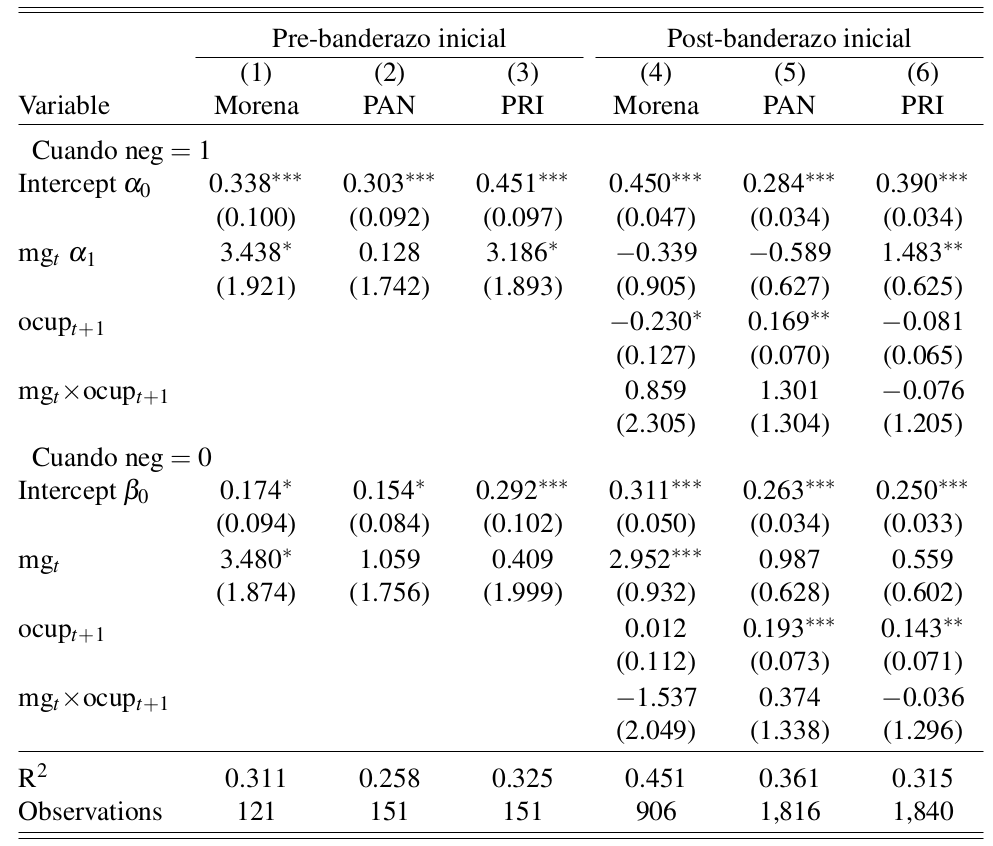
\includegraphics[width=.9\columnwidth]{../../plots/0-ols-table.png}
\end{frame}
\begin{frame}[label={sec:org3146212}]{Replication of Lucardi--Rosas 1997--2017}
\centering
\begin{tabular}{cc}
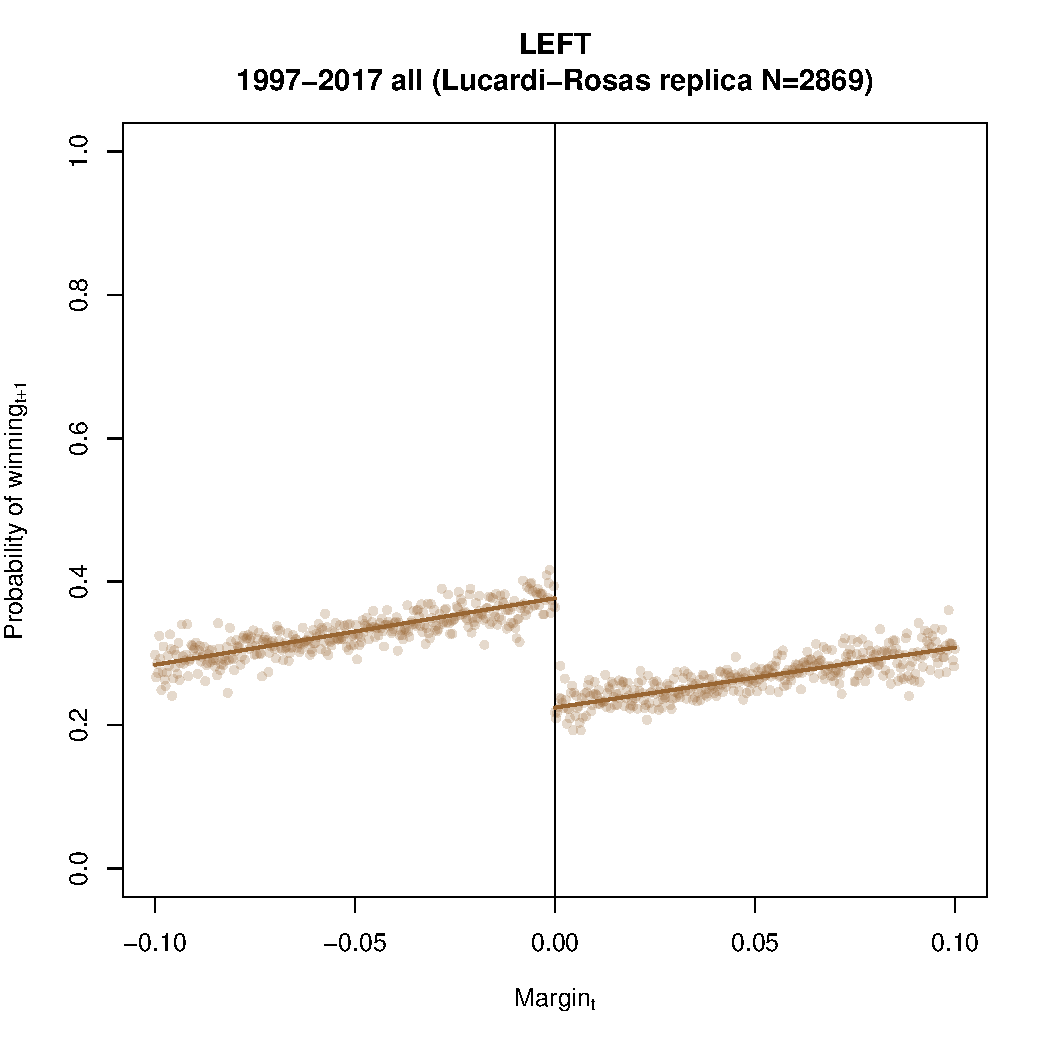
\includegraphics[width=.4\columnwidth]{../../plots/left1REPLICAmcmc.pdf} &
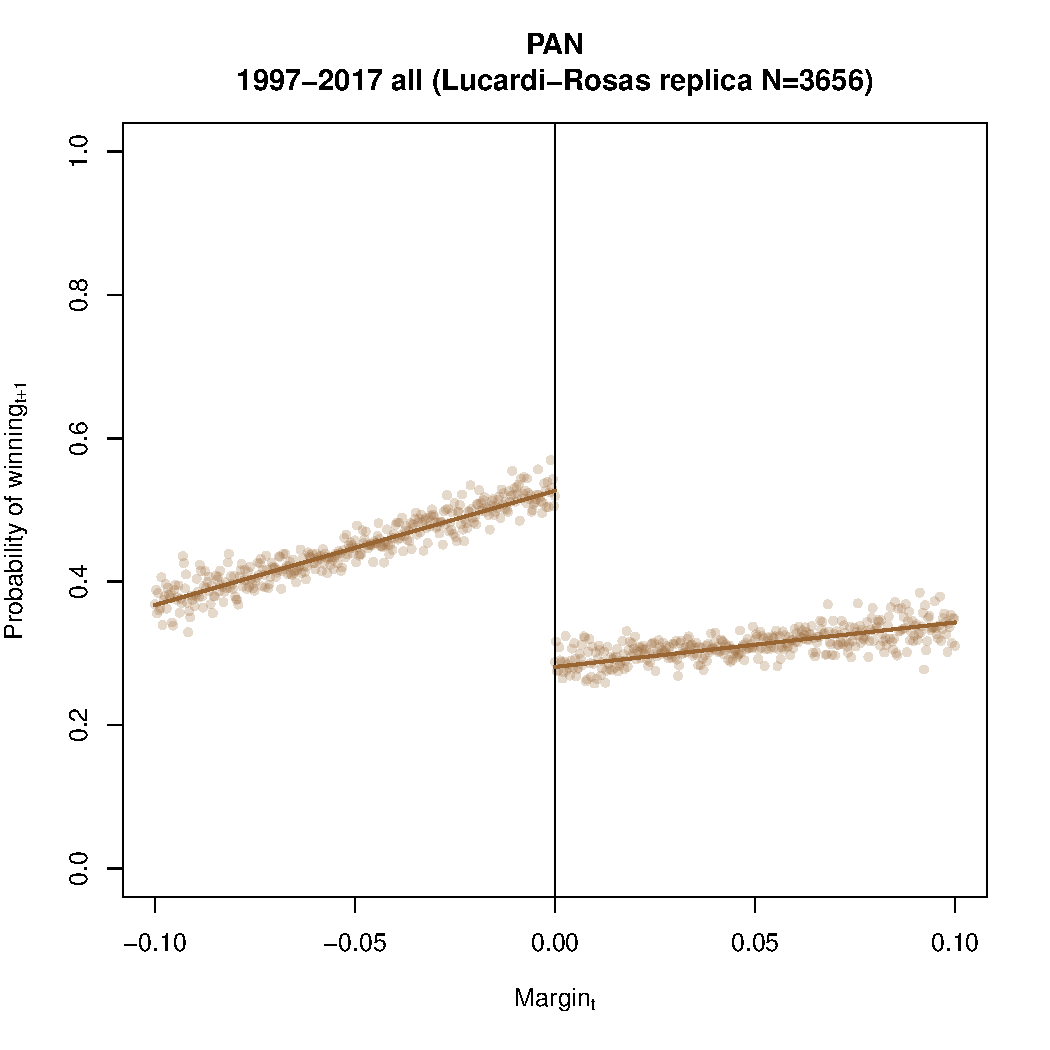
\includegraphics[width=.4\columnwidth]{../../plots/pan1REPLICAmcmc.pdf} \\
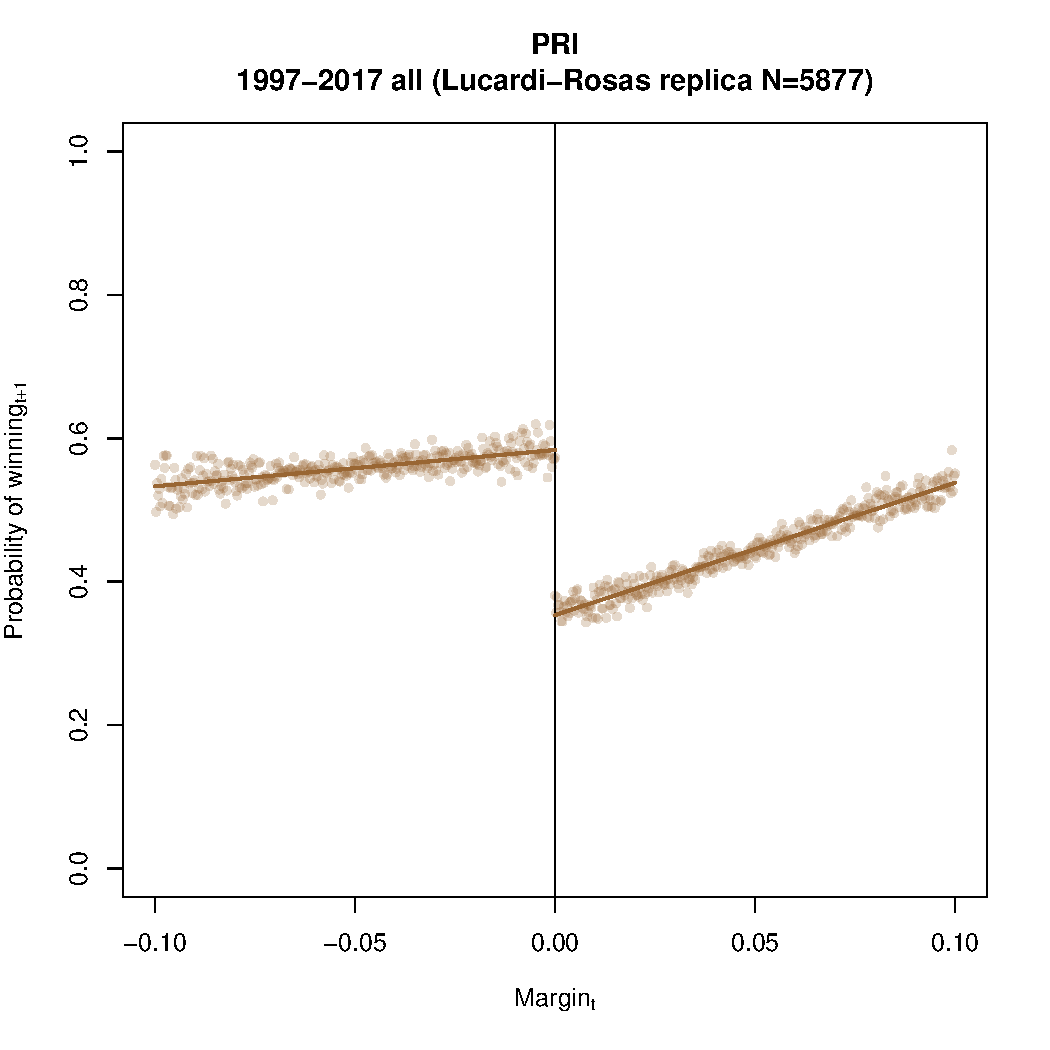
\includegraphics[width=.4\columnwidth]{../../plots/pri1REPLICAmcmc.pdf} \\
\end{tabular}
\end{frame}
\begin{frame}[label={sec:orgc259a07}]{2018--2025 pre-kick-off}
\centering
\begin{tabular}{cc}
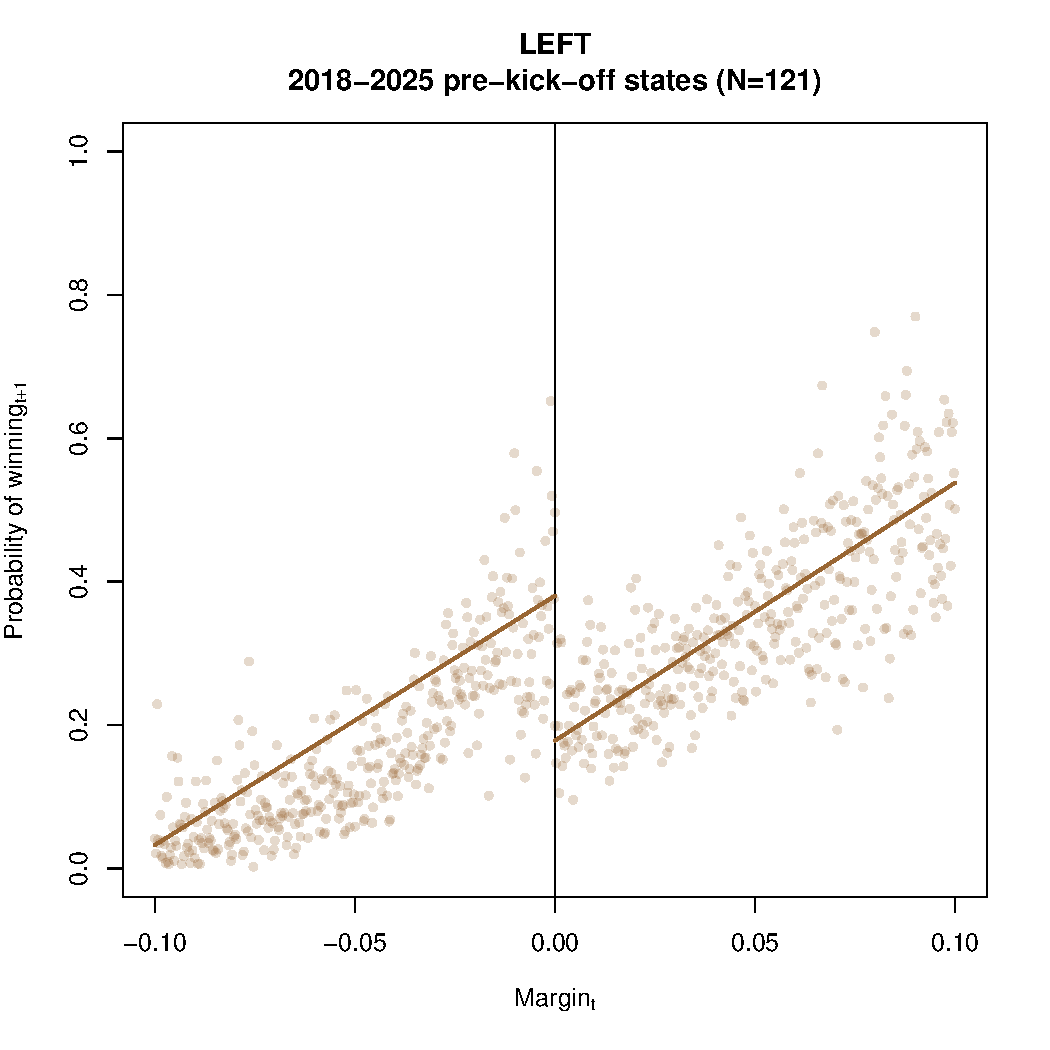
\includegraphics[width=.4\columnwidth]{../../plots/left2PREKICKmcmc.pdf} &
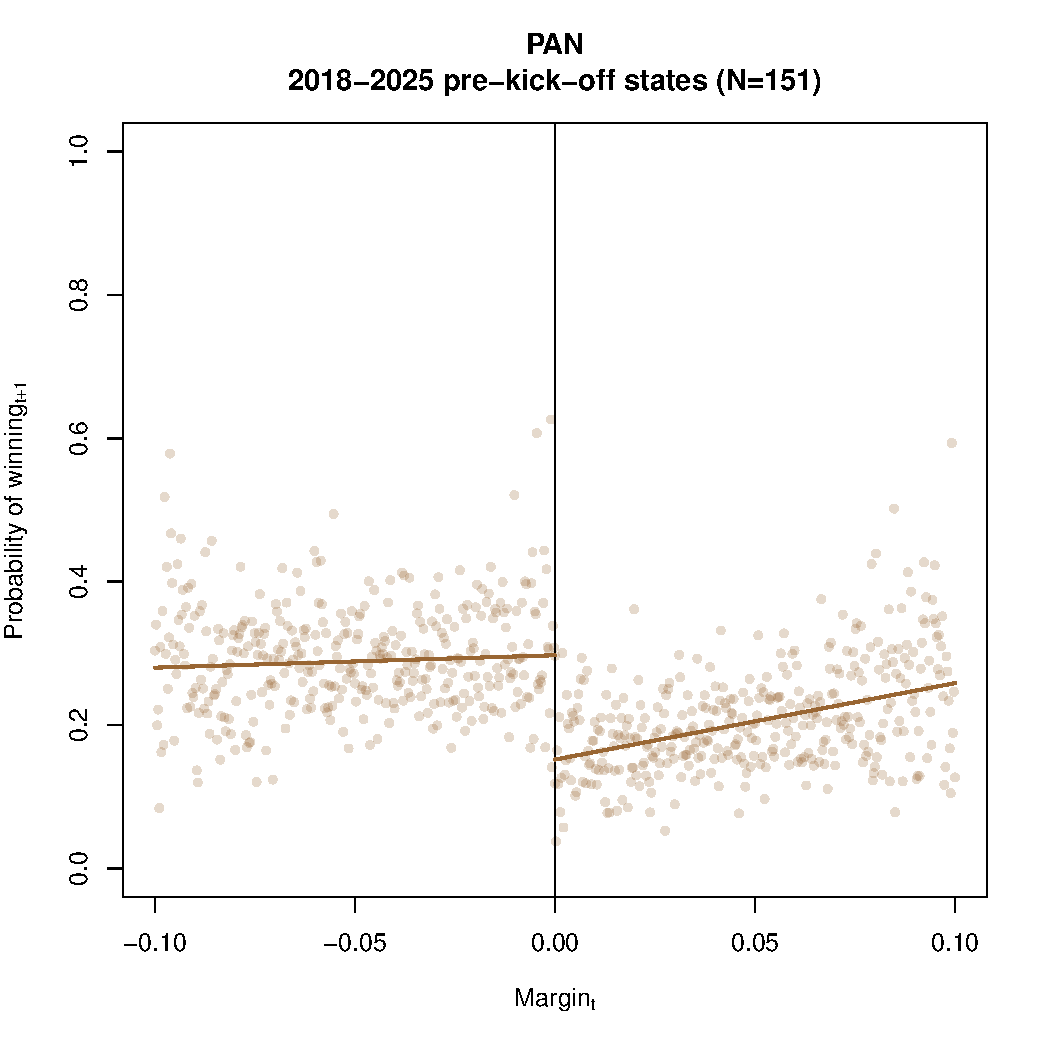
\includegraphics[width=.4\columnwidth]{../../plots/pan2PREKICKmcmc.pdf} \\
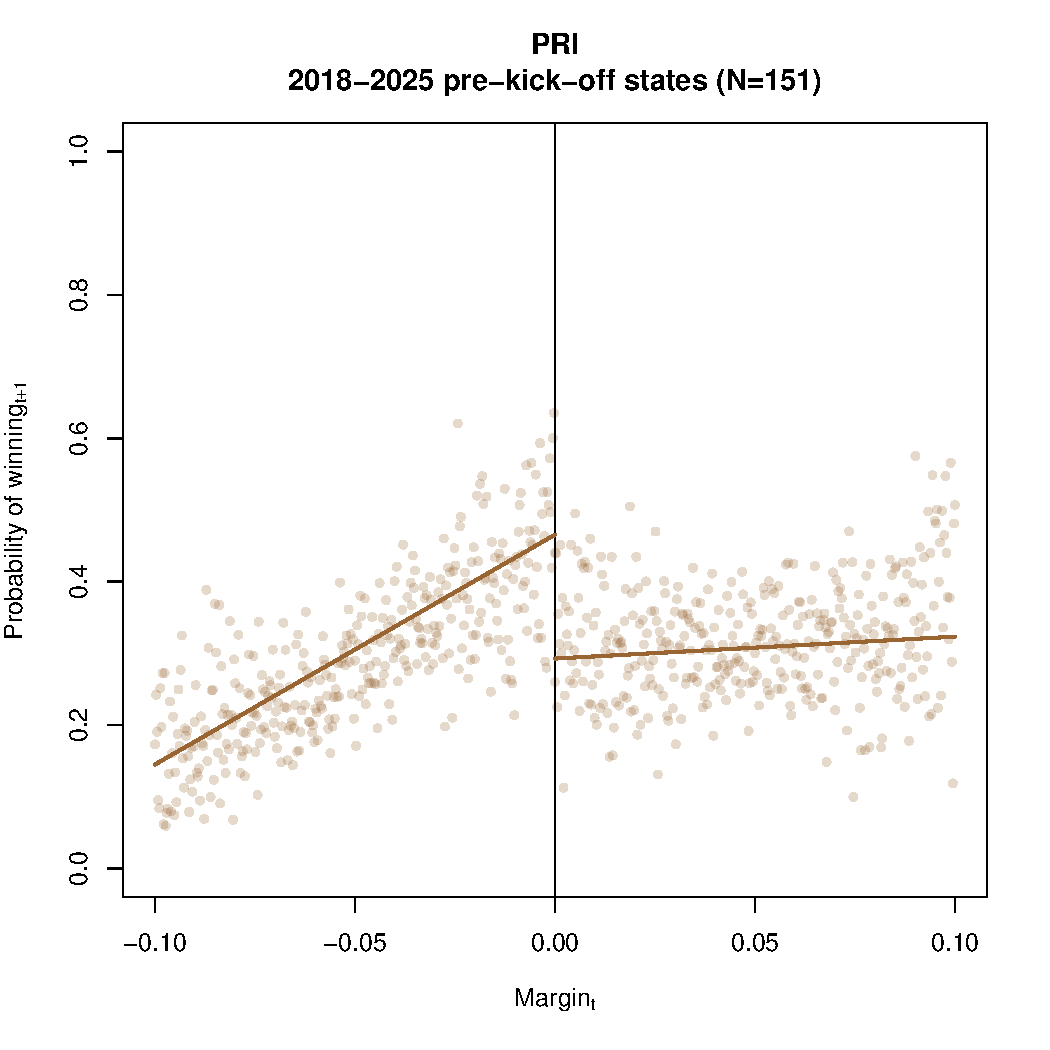
\includegraphics[width=.4\columnwidth]{../../plots/pri2PREKICKmcmc.pdf} \\
\end{tabular}
\end{frame}
\begin{frame}[label={sec:orgeeea210}]{2018--2025 post-kick-off}
\centering
\begin{tabular}{cc}
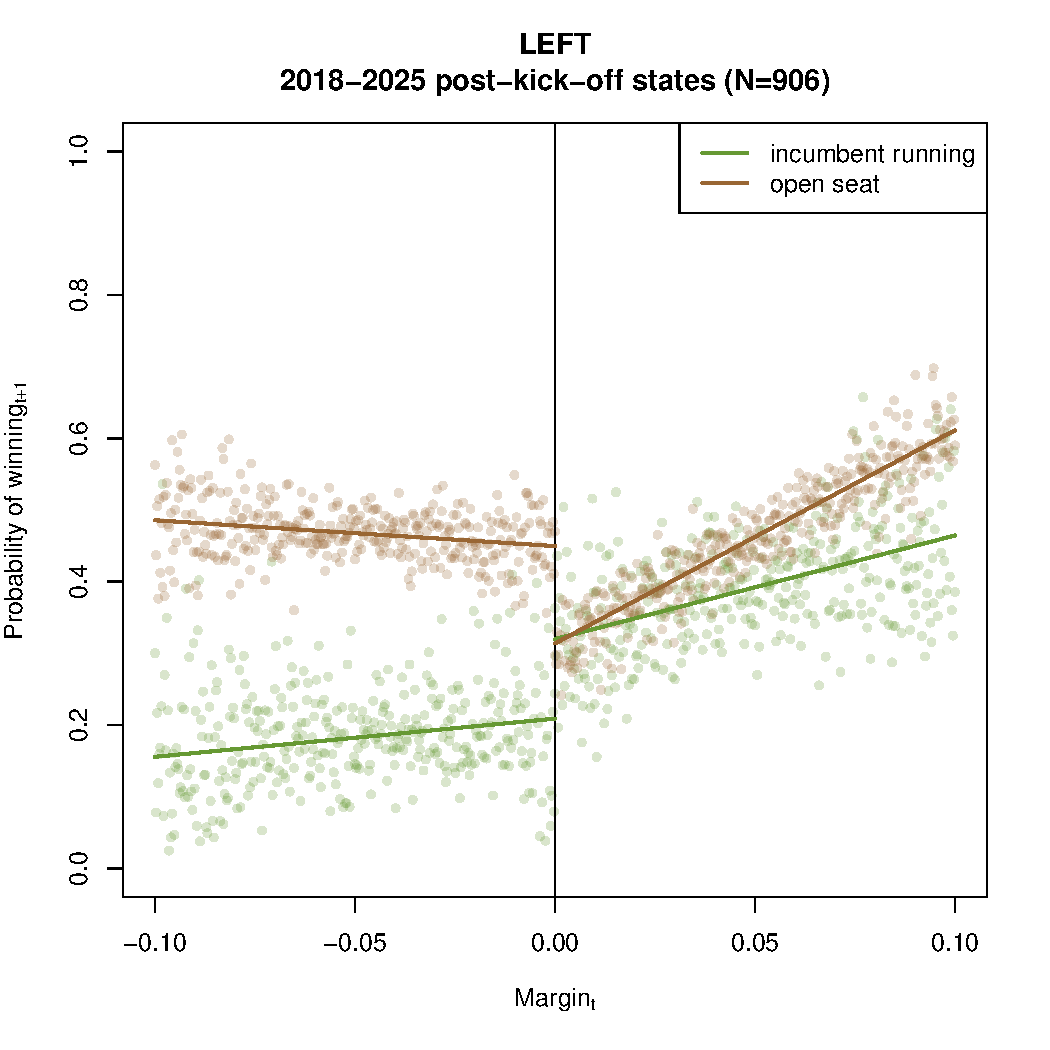
\includegraphics[width=.4\columnwidth]{../../plots/left3POSTKICKmcmc.pdf} &
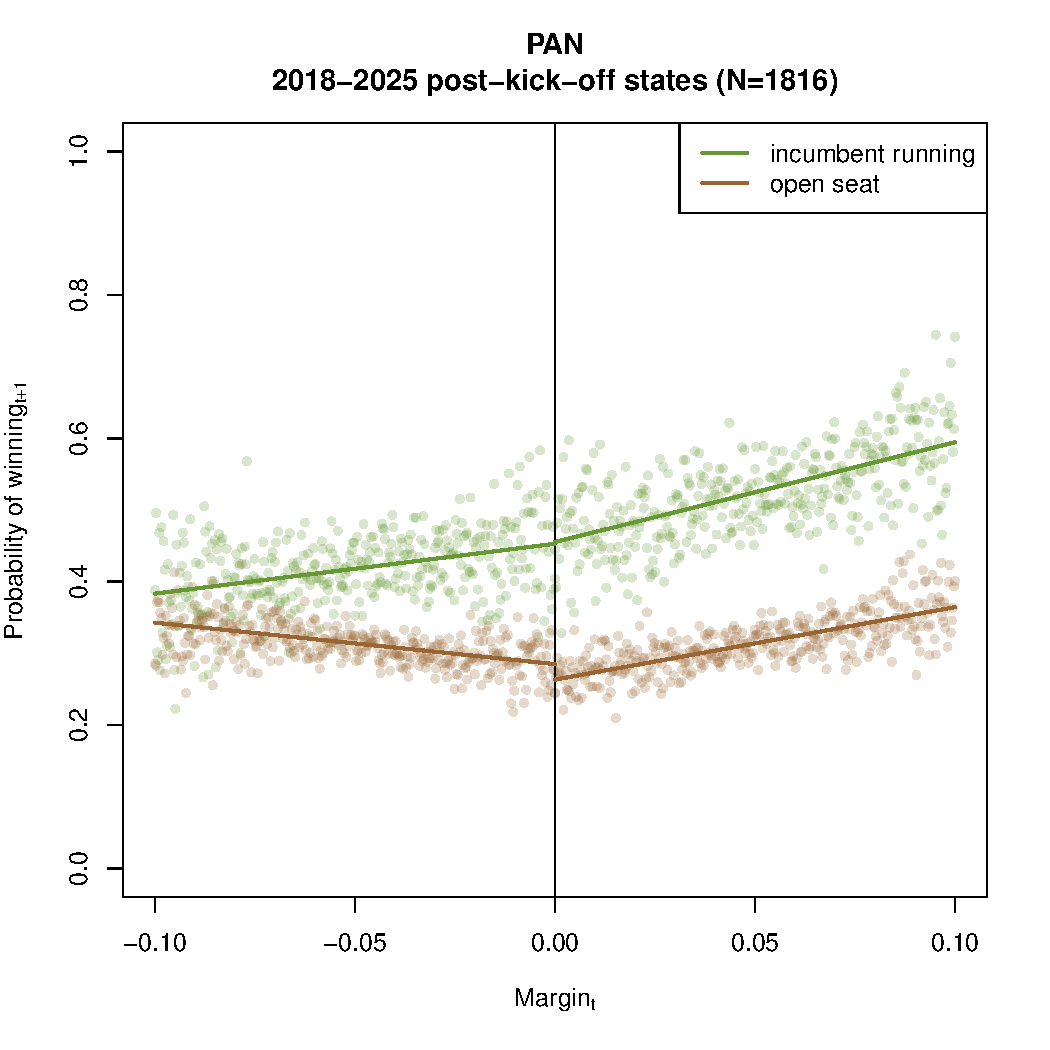
\includegraphics[width=.4\columnwidth]{../../plots/pan3POSTKICKmcmc.pdf} \\
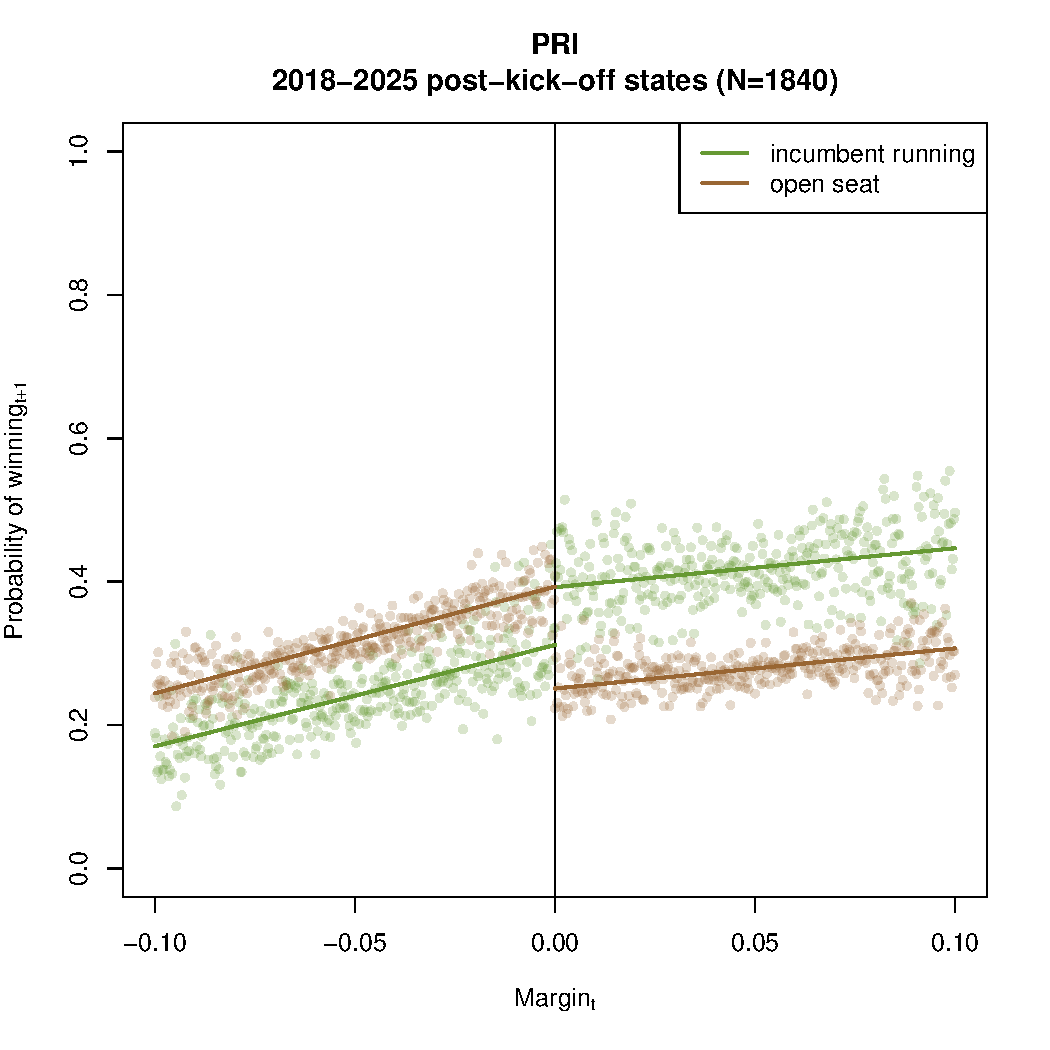
\includegraphics[width=.4\columnwidth]{../../plots/pri3POSTKICKmcmc.pdf} \\
\end{tabular}
\end{frame}
\begin{frame}[label={sec:orgc3f5e83}]{Pooling 1997--2025}
\centering
\begin{tabular}{cc}
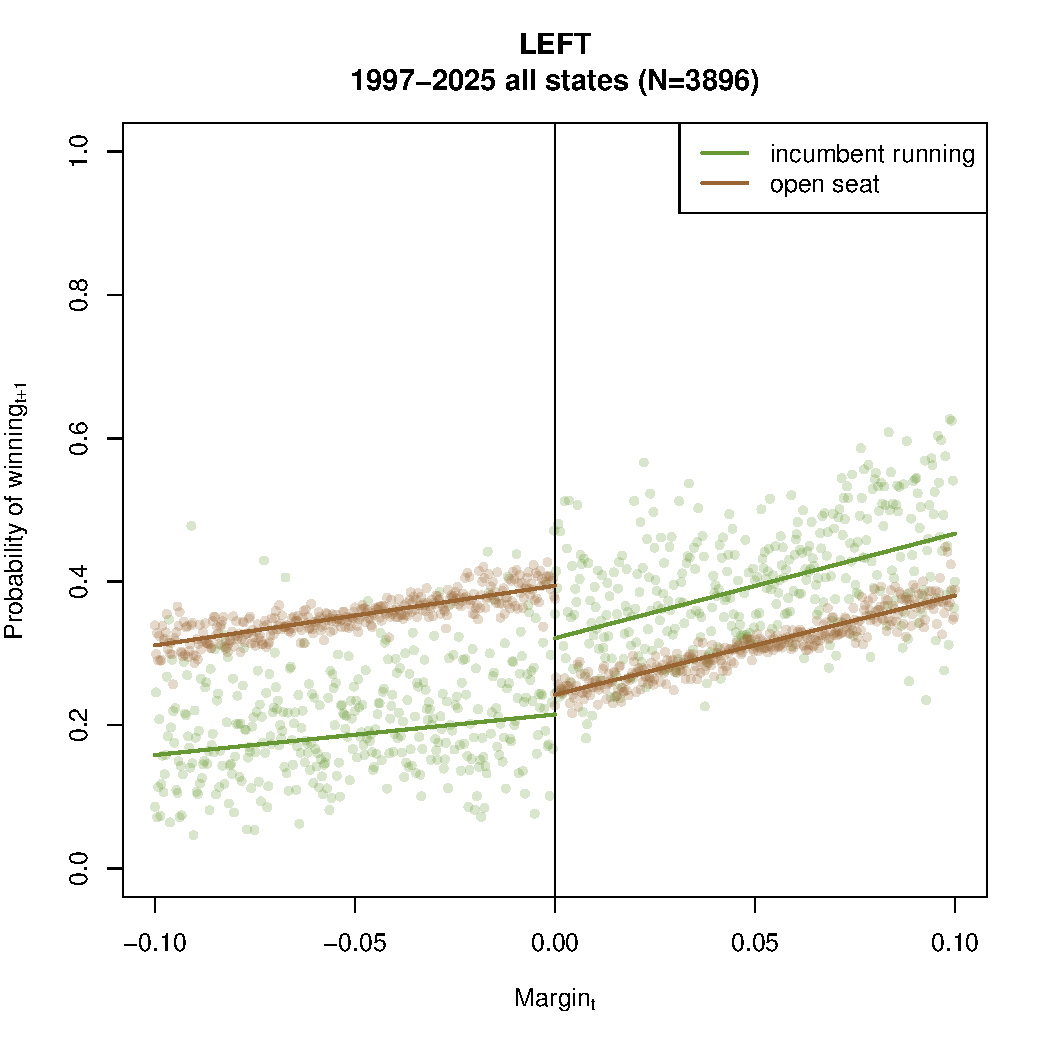
\includegraphics[width=.4\columnwidth]{../../plots/left4ALLmcmc.pdf} &
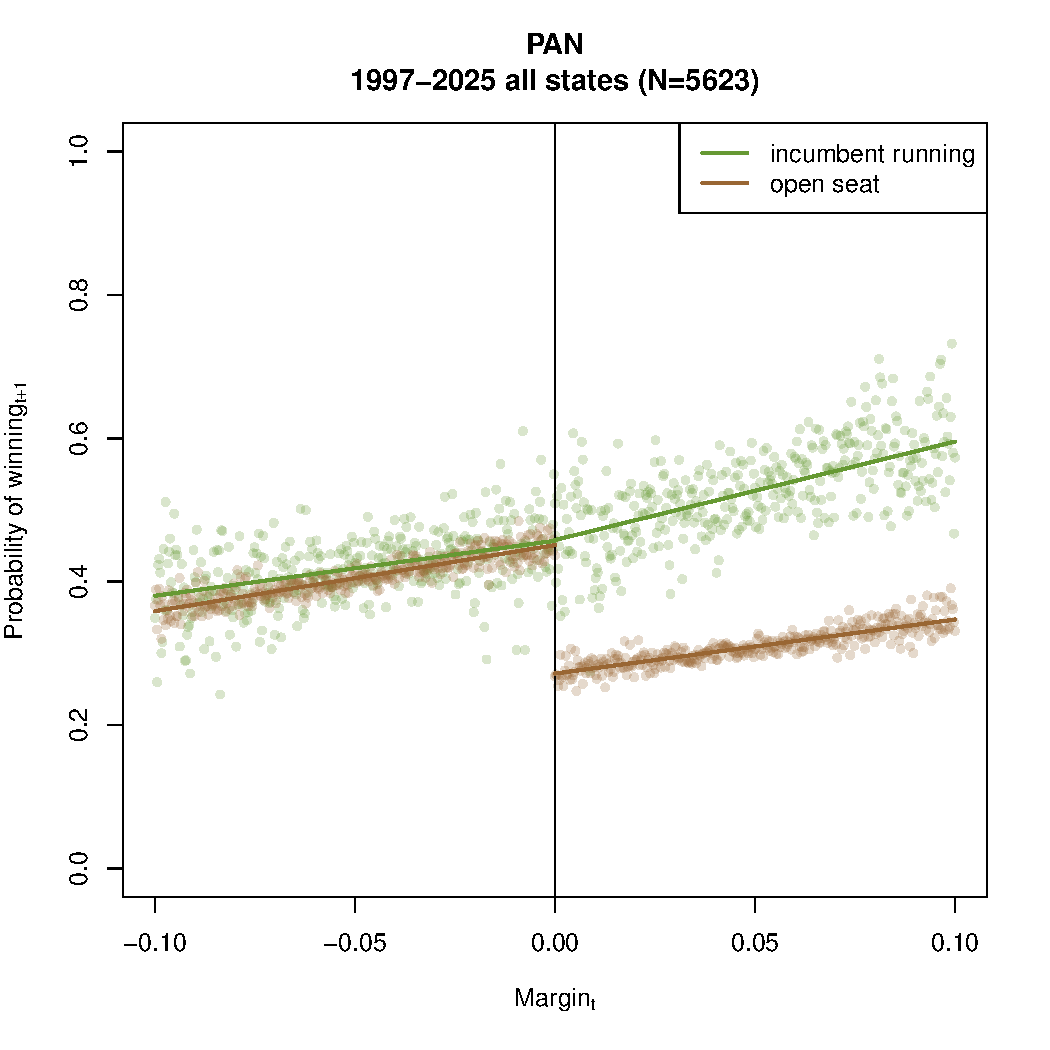
\includegraphics[width=.4\columnwidth]{../../plots/pan4ALLmcmc.pdf} \\
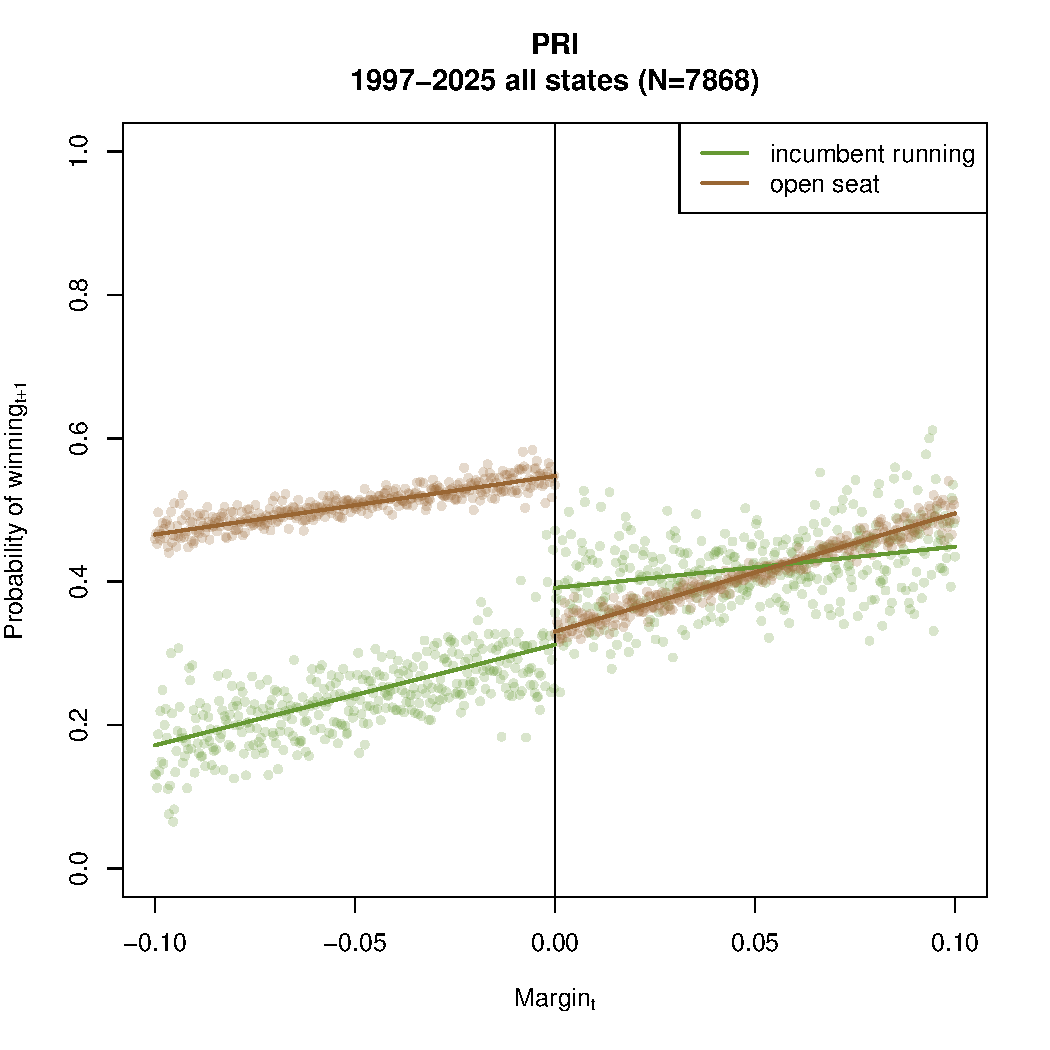
\includegraphics[width=.4\columnwidth]{../../plots/pri4ALLmcmc.pdf} \\
\end{tabular}
\end{frame}
\begin{frame}[label={sec:orgd3ca57a}]{Tests: share of posterior draw conforming with curse hyps.}
\centering \scriptsize
  \begin{tabular}{lccr}
                  &             incumbent ran                   &          not          &       \\
Party & ($\alpha_0 + \alpha_1) > (\beta_0 + \beta_1$) & ($\alpha_0 > \beta_0$) & $N$      \\[-1.5ex] \\ \hline \\[-1.5ex] 
\multicolumn{3}{l}{~\textbf{1997--2017 all municipalities}} \\
Left              &                    ---                      &         1.000         & 2,869 \\
PAN               &                    ---                      &         1.000         & 3,656 \\
PRI               &                    ---                      &         1.000         & 5,877 \\ \\[-1.5ex]
\multicolumn{3}{l}{~\textbf{2018--2025 pre-kick-off municipalities}} \\
Morena            &                    ---                      &         0.916         &   121 \\
PAN               &                    ---                      &         0.876         &   151 \\
PRI               &                    ---                      &         0.858         &   151 \\ \\[-1.5ex]
\multicolumn{3}{l}{~\textbf{2018--2025 post-kick-off municipalities}} \\
Morena            &                    0.219                    &         0.984         &   906 \\
PAN               &                    0.488                    &         0.677         & 1,816 \\
PRI               &                    0.177                    &         0.999         & 1,840 \\ \\[-1.5ex]
\multicolumn{3}{l}{~\textbf{1997--2025 all municipalities}} \\
Left              &                    0.225                    &         1.000         & 3,896 \\
PAN               &                    0.504                    &         1.000         & 5,623 \\
PRI               &                    0.189                    &         1.000         & 7,868 \\[-1.5ex] \\ \hline
  \end{tabular}
\end{frame}
\begin{frame}[label={sec:orge15cfc6}]{Wrap-up}
\begin{itemize}
\item Before kick-off: incumbency curse permeated post-AMLO
\item After: an incumbent running mitigated/inverted it
\item Unlike state assemblies, reform effect is sizeable among municipal executives \newline \(\rightarrow\) mayors with key sources of patronage in spoils system
\item Did counter-reformers kill an insurance policy against negative swings?
\end{itemize}

\centering \bigskip \pause

\textbf{¡Gracias!}
\end{frame}
\end{document}
